\chapter{Analýza lesního mikroklimatu}
\label{chap:ch1}

V následující části \ref{chap:fyz} popíšeme fyzikální děje odehrávající se poblíž zemského povrchu z pohledu mikrometeorologie a mikroklimatologie. Od jednoduchých ilustračních příkladů se přesuneme k tomu, jaký vliv má na mikroklima přítomnost vegetace \ref{chap:veg} a topografie \ref{chap:topo}. V závěrečné části této kapitoly \ref{chap:measure} bude popsáno jak meteorologické podmínky ovlivňují teplotu a jak jsou měřeny, a v \ref{chap:sumavabavorskyles} se podíváme na klima typické pro Národní park Šumava a Bavorský les. V kapitole \ref{chap:statistika} jsou popsány statistické metody využité v kapitole \ref{chap:analysis}.

\section{Fyzikální pohled na děje při povrchu země} \label{chap:fyz}
Pro rovný a téměř homogenní povrch, který můžeme omezit zeshora a zespoda rovinnou, platí zjednodušenná rovnice. Tato rovnice vyjadřuje energetickou bilanci\cite{arya2001}

\begin{gather}\label{eq:bilance}
R_N = H + H_L + H_G + \Delta H_S,
\end{gather}

kde $R_N$ je celková bilance záření, $H$ je tok tepla z nebo do atmosféry, $H_L$ je latentní teplo, $H_G$ je tok tepla ze země a $\Delta H_S$ je změna uchovaného tepla za jednotku času na jednotku plochy přes celou hloubku vrstvy. $\Delta H_S$ můžeme také interpretovat jako rozdíl mezi energií dodanou a odevzdanou z vrstvy která nás zajímá. Pak jestliže $\Delta H_S>0$ tak se vrstva ohřívá a pro $\Delta H_S<0$ tak se ochlazuje jelikož $H_{in}<H_{out}$. Na jednoduchém případě jako třeba na obrázku \ref{fig:energy_drylakebed} můžeme vidět vývoj toku energie na povrchu vyschlého jezera. Přes den se povrch ohřívá díky dopadu slunečního záření $R_N>0$, část tepla uniká pod povrch tedy $H_G<0$ a část ohřívá atmosféru, která sama pouze velmi málo absorbuje záření $H<0$. Naopak v noci vyzařuje povrch dlouhovlnné záření a tím se ochlazuje, tedy $R_N<0$, $H$ je téměř nulové, a zahřátá půda zpětně ohřívá povrch, tedy $H_G>0$. Po celou dobu jde o suchý povrch, tedy $H_L=0$\cite{arya2001}. Většinou ovšem nemůžeme měřit přímo jednotlivé toky tepla.

\begin{figure}
	\centering
	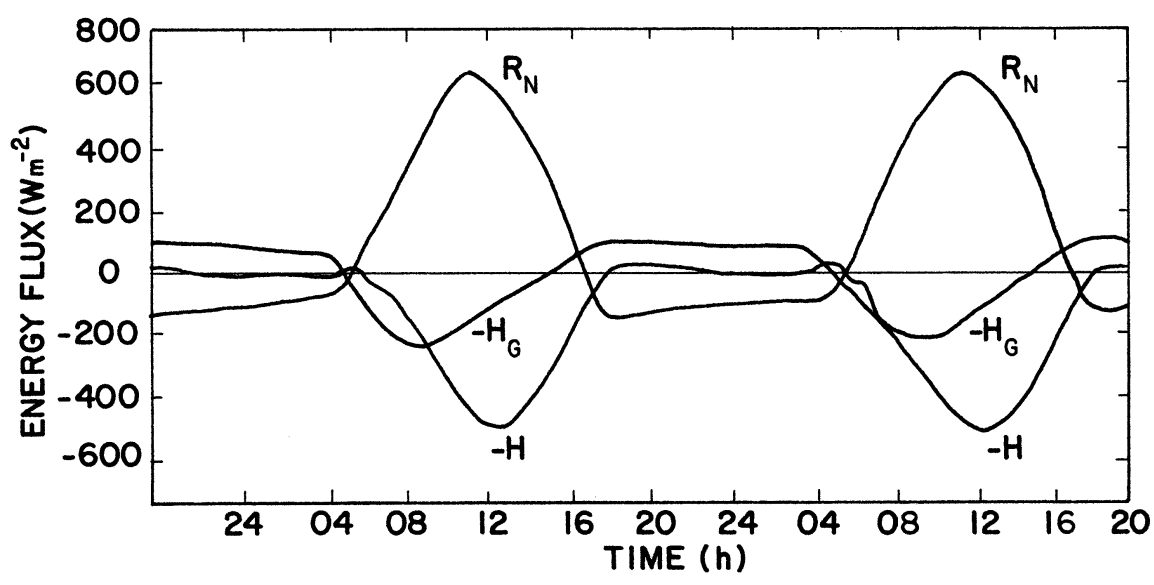
\includegraphics[width=0.95\textwidth]{img/ch1/energy_drylakebed.png}
	\caption{Pozorovaný tok tepla nad vyschlým jezerem El Mirage v Kalifornii 10.-11.6.1950 převzato z \cite{arya2001}}
	\label{fig:energy_drylakebed}
\end{figure}

\subsection{Vliv latentního tepla}\label{chap:latentheat}
Latentní teplo, které značíme $H_L$, je veličina týkající se změny skupenství látek, v našem případě se týká vody. Formálně můžeme latentní teplo zavést jako $H_L = T\Delta s$, kde $T$ je teplota při které dochází ke změně skupenství, a $\Delta s$ je rozdíl mezi molárními entropiemi obou fází\cite{callen1985}. Za standardního atmosférického tlaku $\SI{1013}{hPa}$ je měrné latentní teplo tání $H_{lT} = \SI{334}{kJ/kg}$ a latentní teplo vypařování $H_{lv} = \SI{2265}{kJ/kg}$. 

Výše jsme analyzovali situaci, kdy šlo o suchý povrch. Pro vlhký povrch se nám situace změní. Část tepla bude absorbována vodou a spotřebována na výpar. Můžeme ovšem mít i opačnou situaci, kdy dochází ke kondenzaci vodní páry a uvolňování latentního tepla. Analogicky můžeme uvažovat situaci v zimě, kdy je přítomná voda v pevném skupenství. V našem zjednodušeném příkladě je tedy přes den $H_L > 0$ a v noci $H_L < 0$. Schématicky to můžeme vidět na \ref{fig:schema}, kde velikost jednotlivých toků tepla je ovlivněna mnoha faktory\cite{arya2001}.

\begin{figure}
\centering
	\begin{tikzpicture}
  % Part a: Day
  \draw (-1,0) -- (4,0);
  \draw[pattern=north east lines] (-1,0) rectangle (4,-0.2);
	\draw[-{Stealth},thick] (1,3) -- (1,0) node[midway,left] {$R_N$};
  \draw[-{Stealth},thick] (2,0) -- (2,2) node[midway,right] {$H$};
  \draw[-{Stealth},thick] (3,0) -- (3,1) node[midway,right] {$H_L$};
  \draw[-{Stealth},thick] (0,-0.2) -- (0,-1) node[midway,left] {$H_G$};
  \node at (2,-2) {(a) Situace ve dne};
	\node at (-0.7,0.25) {\textit{Povrch země}};

  % Part b: Night
  \begin{scope}[xshift=6cm]
    \draw (-1,0) -- (4,0);
    \draw[pattern=north east lines] (-1,0) rectangle (4,-0.2);
    \draw[-{Stealth},thick] (1,0) -- (1,1.5) node[midway,left] {$R_N$};
    \draw[-{Stealth},thick] (2,0.75) -- (2,0) node[midway,right] {$H$};
    \draw[-{Stealth},thick] (3,0.5) -- (3,0) node[midway,right] {$H_L$};
    \draw[-{Stealth},thick] (0,-1) -- (0,-0.2) node[midway,left] {$H_G$};
    \node at (2,-2) {(b) Situace v noci};
  \end{scope}
	\end{tikzpicture}
\caption{Schéma toku tepla ve dne a v noci}
\label{fig:schema}
\end{figure}

Vliv vlhkosti a deště můžeme ilustrovat na takzvaném "oázovém efektu". Ve správných podmínkách se může hodnota $H_L$ stát v rovnici \eqref{eq:bilance} i dominantní složkou. Oázovým efektem nazýváme situaci, kdy vítr přináší suchý teplý vzduch přes chladnou a vlhkou oblast. Dochází k silnému výparu, který ochlazuje vlivem latentního tepla povrch země. Následně máme tok tepla $H$ negativní zatímco $H_L$ je větší a pozitivní. Může se stát, že i tok tepla v půdě $H_G$ změní znaménko, pokud povrch bude chladnější než půda. Vlhkost půdy má také vliv na albedo povrchu, způsobuje nárůst absorpce slunečního záření, tedy pokles albeda\cite{arya2001}.

\subsection{Vliv vegetace} \label{chap:veg}
\subsubsection{Albedo}
Albedo je koeficient udávající poměr mezi odraženým a dopadajícím zářením. Albedo nabývá hodnot v intervalu $\langle 0,1\rangle$, kde $0$ znamená, že povrch všechno záření pohlcuje, jde o ideálně černé těleso, a $1$ znamená, že vše záření odráží. Pro situace, kterými se zabývamé v mikrometeorologii, myslíme albedem většinou odrazivost v konkrétním části spektra a to $\SI{0.15}{\micro m}$ až $\SI{4}{\micro m}$. Vyzařování povrchu země se pak týká delších vlnových délek od $\SI{3}{\micro m}$ až $\SI{100}{\micro m}$. 

Už samotný typ povrchu má na albedo významným vliv. Může dosahovat velmi různých hodnot ať už jde o písek, vodní plochu, odhalenou půdu, vlhkou půdu atd. Růst vegetace a jejího typu má ovšem také významným vliv na albedo s odlišnými hodnotami pro různé typy plodin a různé typy dřevin. Ilustrační příklady jsou vidět v tabulce \ref{tab:albedo}. Hodnoty jsou závislé i na úhlu dopadu záření, vliv má i výška porostu nebo roční období\cite{arya2001,alma}.

\begin{table}
\centering\footnotesize\sf
\begin{tabular}{lr}
\toprule
Typ povrchu & Albedo \\
\midrule
Vodní plocha & 0.10-1.00 \\
Čerstvý snih & 0.45-0.95 \\
Suchý písek & 0.35-0.45\\
Vlhký písek & 0.2-0.3\\
Krátký trávník ($\SI{20}{cm}$) & 0.26\\
Delší trávník ($\SI{1}{m}$) & 0.16\\
Opadavý les & 0.1-0.2\\
Neopadavý les & 0.05-0.15\\
\bottomrule
\end{tabular}
	\caption{Výběr různých typů povrchů a odpovídajících hodnot albeda. Převzato z \cite{arya2001}.}
\label{tab:albedo}
\end{table}

\subsubsection{Vliv na tok tepla}
Do členů v rovnici \ref{eq:bilance} můžeme zahrnout i růst vegetace. V tu chvíli musíme počítat s významnou prostorovou závislostí všech toků tepla a záření. Následně jsou pro nás nejdůležitější hodnoty $R_N$, $H$ a $H_L$ nad vegetací. $\Delta H_S$ se skládá ze dvou částí a to změna tepla ve vzduchu, vegetaci, atp., a změna energie biochemického původu skrze fotosyntézu a přesunu oxidu uhličitého. Latentní teplo se pak skládá z výparu a kondenzace vody a také z transpirace vody listy rostlin, mluvíme pak o evapotranspiraci\cite{arya2001}. 

Vliv na celkový tok energie má i výška porostu, například v lese může být nezanedbatelné množství tepla uchovaného v úrovni vegetace, které může způsobit, že prostředí reaguje pomalu na změnu teploty a jiných veličin. Pro suchý porost může uchovaná energie dosahovat až $\SI{7}{\%}$ celkového toku energie skrz dopadající záření, situace se ovšem pro vlhký porost obrací, a denní uchovaná energie může být záporná\cite{alma}. 

Podle \cite{alma} ovlivňuje teplotu hustota porostu. Měříme-li teplotu v řidším lese, a sledujeme její průběh od země až po koruny stromů, tak teplo snadněji prochází vegetací. Při zemi tedy budou podobné teploty jako ve výšce několika metrů nebo až v korunách stromů. Naopak, pokud se nacházíme v hustějším lese, tak bude teplota růst dříve v oblasti korun stromů a teplota při zemi může mít zpoždění několik hodin a také nižší denní maximální hodnoty. V noci také může v řidším lese docházet k inverzi teplot, zatímco v hustějším lese budou teploty podobné napříč porostem. 

Tok tepla v lese je ovlivněn i větrem. Jestliže fouká silný vítr, dochází k rychlému přenosu tepelné energie mimo lesní porost\cite{alma}. 

\subsubsection{Vliv na rychlost větru}\label{chap:vlivnavitr}
Turbulence vzduchu je zodpovědná za přenos hmoty, tepla a hybnosti v blízkosti povrchu země. Bez turbulence by promíchávání probíhalo na molekulární úrovni a řádově menším měřítku. Na míru turbulence a promíchávání má vliv rychlost větru. Vegetace ovlivňuje nejen rychlost větru, ale také její profil. Například koruny stromů můžou rychlost větru výrazně snižovat. Zatímco rychlost větru zde může být vyšší, pokud blízko země nejsou menší stromy, keře nebo jiné překážky. To má pak vliv na teploty uvnitř porostu, které se mohou více podobat teplotám ve volném vzduchu. Tímto je zřejmé, že vliv na rychlost větru má i přítomnost listů a jejich absence v zimě \cite{alma}. 

\subsubsection{Vliv na vlhkost vzduchu}
V předchozím odstavci jsme zmínili transpiraci flóry, která slouží jako zdroj vodní páry. Ukázková situace v jehličnatém lese může vypadat tak, že tlak vodní páry dosahuje dvou maxim a to při povrchu půdy z důvodu nižšího promíchávání vzduchu a výparu a v oblasti korun stromů kvůli listům. Druhé maximum bývá ovšem menší, kvůli promíchávání se suchým vzduchem nad korunami stromů. Vzhledem k absolutním rozdílům tlaku vodních par v řádu jednotek milibarů, změna relativní vlhkosti napříč dnem a výškou je dána především teplotním zvrstvením \cite{alma}. 

\subsubsection{Vliv na rosu}
Stromy nejenže stíní povrch země před přímým slunečním zářením a ovlivňují vyzařování dlouhovlnného záření povrchem, ale také ovlivňují množství rosy. Při měření množství ranní rosy v různé vzdálenosti od kmene stromu bylo pozorováno, že množství rosy roste strmě do zhruba $\SI{2}{m}$ od kmene a dále pomaleji. Doba, po kterou zůstala rosa na zemi, také se vzdáleností rostla a od vzdálenosti $\SI{4}{m}$ lehce klesala \cite{alma}.

\subsubsection{Vliv na déšť}
Listnaté, ale i jehličnaté stromy mají vliv na distribuci deště. Největší množství vody se objevuje na vnějším okraji ohraničeném korunou stromu. Stromy bez listů mají na prostorové rozložení srážek pouze minimální vliv. Pod jehličnaté stromy dopadá pouze $\SI{60}{\%}$ až $\SI{90}{\%}$ srážek, a v oblasti okraje korun dopadá o $\SI{10}{\%}$ až $\SI{20}{\%}$ více srážek než v místě bez porostu. Lesní porost také při slabém dešti může úplně zabránit dopadu srážek na půdu. Množství vody, které takto dokážou stromy zachytit, se může pohybovat od $\SI{1}{mm}$ do $\SI{3}{mm}$. Část vody je také ztracena výparem z povrchu listu, který je podpořen výraznějším promícháváním vzduchu v oblasti horní části korun stromů \cite{alma}.

\subsubsection{Vliv na sníh}
Množství sněhový srážek, které dopadnou na zem v lesním porostu záleží na několika faktorech. Jestliže jde o mokrý sníh, pak snadno zůstává v korunách stromů, takto může být v korunách zachyceno až $\SI{10}{cm}$ sněhu. Suchý sníh naopak snáze dopadne na zem. Množství zachyceného sněhu závisí také na typu vegetace, jestli jde o listnaté nebo jehličnaté stromy, případně o jaký druh. Na jaře taje sníh v lese pomaleji a jeho přítomnost je pro místní klima velmi důležitá, jelikož funguje jako zásobník vody\cite{alma}.

\subsection{Vliv topografie} \label{chap:topo}
V odstavcích výše bylo vysvětleno, jakým způsobem může ovlivnit vegetace podnebí. Bylo ilustrováno, že přítomnost flóry má významný vliv na celou řadu meteorologických proměnných, které následně ovlivňují teplotu v lese a život organismů. Nyní se budeme soustředit na vliv topografie na meteorologické proměnné. Pro standardizované meteorologické stanice je typické, že jsou postavené na posekané travnaté ploše, která není zastíněná a terén není nakloněn, v reálné krajině tohle ovšem neplatí.

\subsubsection{Vliv okraje lesa}
V oblasti okraje lesního porostu máme kontakt rozhraní dvou rozdílných vzduchových hmot. Geografická orientace má vliv na to, jak dlouho svítí denní světlo na toto rozhraní. Množství dopadající energie může být pro okraj lesa orientovaný na jih i několikrát větší, než pro okraj orientovaný na sever. To platí například pro lesy v Evropě. Na rozhraní lesa a otevřené oblasti můžeme dokonce pozorovat vyšší teploty než uvnitř lesa a mimo něj, částečně to může být kvůli sníženému promíchávání vzduchu, větší absorpci slunečního záření, stínění dlouhovlnného záření a nižšímu výparu. Vliv na teplotu má i vítr. Jestliže fouká směrem do lesa, pak je tendence, aby teplota na okraji lesa byla podobná teplotě mimo les a naopak pro vítr směrem z lesa\cite{alma}.

\subsubsection{Vliv sklonu a orientace svahu}
Množství slunečního záření, které dopadne na povrch země závisí na mnoha faktorech. Musíme vzít v potaz zeměpisnou šířku, období v roce, denní čas, sklon svahu a orientaci svahu. Například pro svah s velkým sklonem na severní polokouli, který míří na sever, se může stát, že v zimě nedostane po většinu dne žádné sluneční záření. Abychom dostali úplný obrázek musíme započítat i difúzní záření, které je primární složkou záření, pokud je zataženo. Difúzní záření není do takové míry ovlivněné sklonem svahu\cite{alma}.

\subsubsection{Vliv údolí}
Nejen sklon a orientace svahu mají vliv na mikroklima. Jeden z dalších důležitých aspektů je jestli se místo, kterým se zabýváme, nachází v údolí nebo, zda-li jde o kopec. Topografie údolí má vliv hned několika způsoby. Studený vzduch je hustší a tudíž klesá do údolí, kde pak může vznikat kapsa studeného vzduchu. Údolí je typické prostředí, kde můžeme pozorovat inverzi vzduchu. Údolní topografie může způsobovat to, že na dno dopadá menší množství slunečního záření, zároveň je ale dlouhovlnné záření částečně stíněno okraji údolí. Do údolí hůře proniká vítr, a tudíž je zde snížená turbulence a tím i turbulencí předávané teplo, viz \ref{chap:vlivnavitr}. Pro velmi úzké a hluboké propadliny je půda významným zdrojem tepla. Všechny tyto faktory mají opačný vliv v případě kopců a obecně vyvýšených míst\cite{alma}. 

\subsubsection{Vliv topografie na vítr}
Vítr ovlivněný topografií terénu můžeme rozdělit na tři typy podle původu: kompenzační vítr, horský a údolní vítr a vítr spojený se sklonem svahu. V prvním případě jde o vítr způsobený nevyváženým ohřevem zemského povrchu. Na teplejším místě se izobary začnou zvedat, a tím vzniká horizontální gradient tlaku mezi chladnou a teplejší oblastí. Vítr spojený se sklonem svahu má v noci tendenci jít z vyšších nadmořských poloh dolů a naopak během dne. Můžeme mít také situaci, kdy pozorujeme údolí, které se zároveň svažuje. Zde už je situace složitější.

Při svítání se začíná povrch údolí ohřívat. Vzduch u strany údolí stoupá nahoru, ale údolní vítr stále ještě fouká směrem dolů. Během dne údolní vítr oslabuje, až dojde k obrácení jeho směru a údolím fouká nahoru. Později odpoledne vítr po svazích začne ustávat, a fouká pouze údolní vítr do vyšších nadmořských výšek. Následně chladnější vzduch ze stran údolí začne klesat, a v noci nakonec údolní vítr začne opět vát dolů stejně jako vítr po svazích údolí. Toto popisuje ukázkovou situaci za letního dne bez oblačnosti. Ilustraci k tomuto popisu můžeme vidět na obrázku \ref{fig:valley_winds}

\begin{figure}
	\centering
	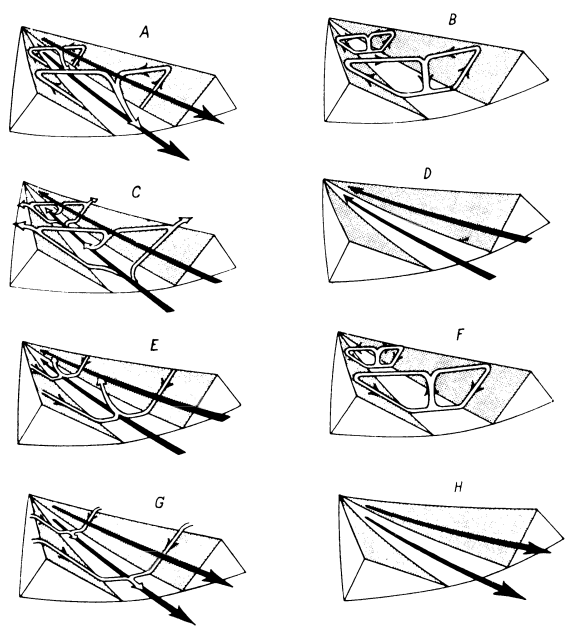
\includegraphics[width=0.95\textwidth]{img/ch1/valley_winds.png}
	\caption{Typický průběh proudění napříč letním dnem. Převzato z \cite{alma}.}
	\label{fig:valley_winds}
\end{figure}

Vítr ovlivněný topografií může mít další podoby, které ovšem pro tuto práci nejsou zásadní. Můžeme zmínit mořský vánek mezi střídavě rychle se ohřívajícím pobřežím a relativně studenému moři ve dne, a rychle chladnoucím pobřeží a relativně teplému moři v noci. Významný vítr spojený s horskou topografií pak dostává různé názvy jako fén v Alpách nebo mistrál ve Francii\cite{alma}.

\subsection{Rozdíl mezi teplotou při povrchu země a ve standardní výšce}
Teplotou ve standardní výšce se typicky myslí ve výšce $\SI{1}{m}-\SI{2}{m}$. Jestliže máme situaci, kdy na povrch svítí přímé sluneční záření, tak se můžou vyskytovat výrazné gradienty teplot a to až $\SI{10}{K/mm}-\SI{20}{K/mm}$. Tyto výrazné gradienty jsou ovlivněné mnoha faktory jako například druh povrchu nebo jeho vlhkost a další, jak bylo diskutováno výše. Dále kvůli nezanedbatelné velikosti teplotních senzorů je netriviální měřit teplotu povrchu\cite{arya2001}. 

\section{Analýza faktorů ovlivňující teplotu vzduchu v lesním porostu}
V předchozích odstavcích jsme diskutovali vliv vegetace a topografie na různé meteorologické proměnné. Tuto souvislost v následující části budeme diskutovat na konkrétní studii týkající se výzkumu ploch po střední Evropě.

\subsection{Vliv topografie a struktury krajiny na teplotu}
Při hledání vlivu topografie na rozdíl mezi teplotou v lesním porostu a na nejbližší meteorologické stanici ve střední Evropě byly ve výzkumu \cite{ZellwegerFlorian2019Sdou} použity následující prediktory.

\begin{itemize}
	\item Plocha pokrytá lesním porostem v okruhu $\SI{250}{m}$ vyjádřená v procentech. Zde nebyla nalezena spojitost s rozdílem teplot.
	\item Vzdálenost k okraji lesa byla nevýznamným prediktorem. 
	\item Vzdálenost k nejbližšímu pobřeží a výška nad mořem byly nejsilnějšími prediktory, zároveň jde ovšem o silně korelované veličiny. Slabšími prediktory pak bylo stočení svahu k severu/jihu, sklon svahu a hodnota udávající zda-li jde spíše o údolí nebo vyvýšené místo.
\end{itemize}

Tyto výsledky ovšem nejsou nutně konzistentní mezi různými studiemi. Například podle \cite{GreiserCaroline2018Mmmi} je plocha pokrytá lesním porostem důležitou hodnotou a může vést ke zvýšení minimální denní teploty až o $\SI{3}{\degree C}$, nebo vzdálenost k okraji lesa je středně silný prediktor.

\subsection{Vliv porostu na teplotu}
Druhou skupinou prediktorů, kterou se \cite{ZellwegerFlorian2019Sdou} zabýval, byly proměnné týkající se porostu v blízkém okolí čidla.

\begin{itemize}
	\item Zápoj má pro hodnoty nižší než $\SI{89}{\%}$ záporný vliv, pro vyšší hodnoty pak neutrální až lehce kladný vliv.
	\item Otevřenost porostu vyjádřená jako část viditelné oblohy a plocha koruny stromů má také záporný nelineární vztah k maximální teplotě.
	\item Procento plochy pokryté dřevinami nad určitý průměr je pouze slabým prediktorem. 
	\item Výška stromu, na kterém bylo čidlo upevněno, naopak souvisí s rozdílem maximální teplot kladně, ale opět zde vztah není příliš silný.
	\item Schopnost porostu vytvářet stín podle typu dřeviny je středním prediktorem rozdílu maximálních teplot.
\end{itemize}

\subsection{Vliv meteorologických podmínek na teplotu}
Jak bylo zmíněno v předchozí části, tak na rozdíl mezi teplotou mimo porost a v lese má vliv mnoho faktorů od topografických po konkrétní typ porostu. Tyto faktory se dají vyjádřit mnoha různými prediktory, jejichž vliv můžeme sledovat. Aktuální stav počasí je ovšem další faktorem, který ovlivňuje naměřené teploty. Tím může být oblačnost, vlhkost, sněhová pokrývka, srážky, rychlost větru a insolace. Vybrali jsme si tyto, protože s nimi budeme pracovat v kapitole \ref{chap:analysis}.

Při zvýšené oblačnosti dopadá na zem více rozptýleného záření a povrch země se neohřívá přes den tak rychle, stejně tak ovšem oblačnost přes noc zabraňuje úniku dlouhovlnného záření, a tedy obecně snižuje amplitudu denního chodu teplot. Tento pokles můžeme vidět na obrázku \ref{fig:diurnaltemp}\cite{arya2001}.

\begin{figure}
	\centering
	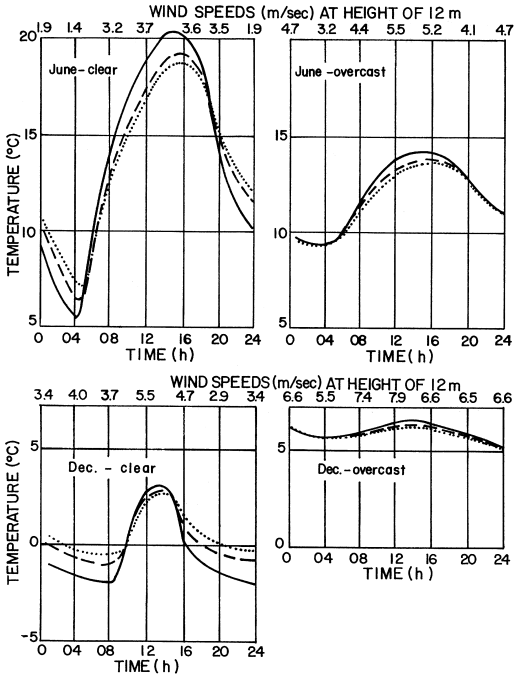
\includegraphics[width=0.95\textwidth]{img/ch1/diurnaltemp.png}
	\caption{Denní vývoj teploty ve třech výškách (plná čára $\SI{1.2}{m}$, čárkovaná $\SI{7}{m}$ a tečkovaná $\SI{17}{m}$) v jižní Anglii pro jasnou a zataženou oblohu a pro červnové a prosincové teploty. Převzato z \cite{arya2001}}
	\label{fig:diurnaltemp}
\end{figure}

Vítr napomáhá promíchávání ohřívaného vzduchu u zemského povrchu s vyššími vrstvami, a tedy typicky dochází při silnějším větru k poklesu teplotního gradientu nad zemí\cite{arya2001}.

Sníh má nízkou tepelnou vodivost. Pod sněhovou pokrývkou tedy v zimě typicky dochází k nárůstu teplot. Zatímco na povrchu sněhu můžou teploty klesat hluboko pod bod mrazu, sníh izoluje zemský povrch. Studie z oblasti Altajského pohoří pozorovala rozdíl teplot mezi zemským povrchem a horní hranicí sněhové pokrývky (o výšce $\SI{0.5}{m}$) až $\SI{12.8}{\degree C}$. Tuto skutečnost, kterou využívají pro přežití zimy různé organismy\cite{hirakawahirofumi2018}, můžeme vidět na obrázku \ref{fig:snowtempaltai}. Zatímco na rozhraní vzduch-sníh kolísají teploty od $\SI{0}{\degree C}$ téměř k $\SI{-30}{\degree C}$, tak s hloubkou nejenže amplituda dramaticky klesá, ale také jsou teploty bez výjimky vyšší. Dále můžeme vidět, že výkyvy teplot, ať už dané denním chodem nebo změnou počasí, mají ve sněhové pokrývce zpoždění, které se prodlužuje s výškou sněhu\cite{zhangwei2021}. 

\begin{figure}
	\centering
	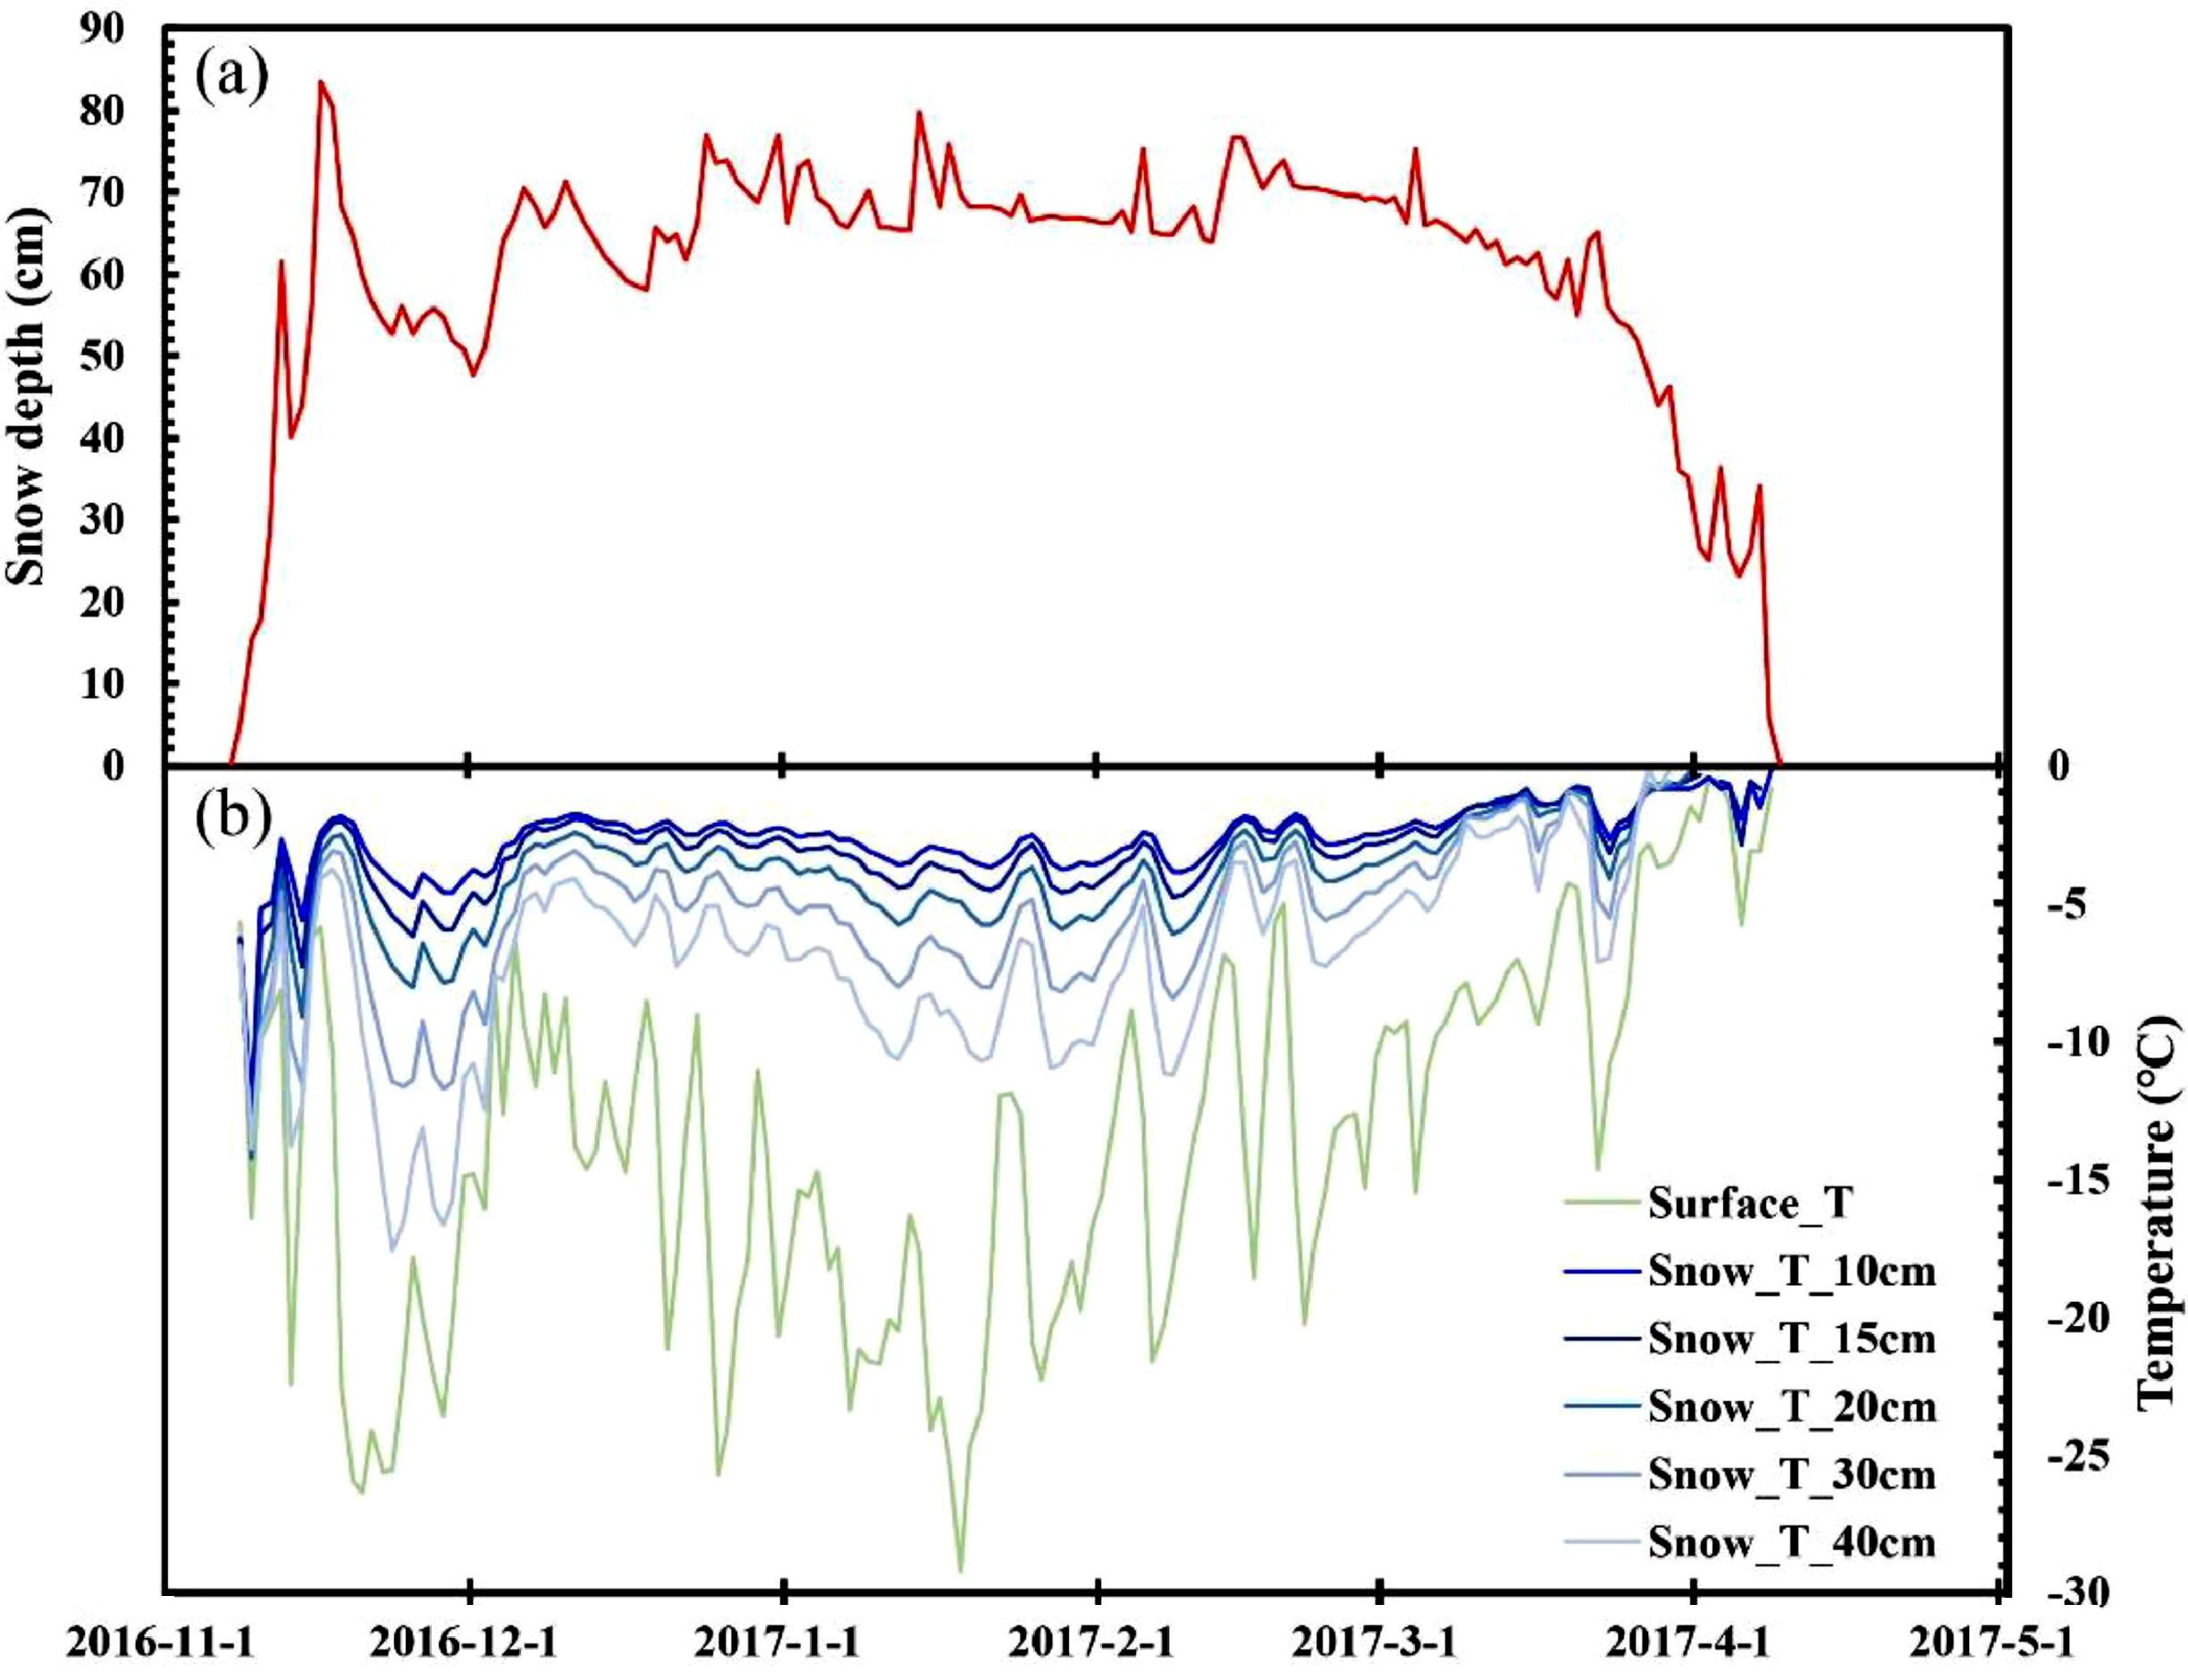
\includegraphics[width=0.95\textwidth]{img/ch1/snowtempaltai.png}
	\caption{Sezónní vývoj teplot pod sněhovou pokrývkou pro $\SI{10}{cm}$, $\SI{15}{cm}$, $\SI{20}{cm}$, $\SI{30}{cm}$, $\SI{40}{cm}$ nad rozhraním půda-sníh a na povrchu sněhu. Data se týkají období od listopadu 2016 do dubna 2017 pozorovaných na Altaji. Převzato z \cite{zhangwei2021}.}
	\label{fig:snowtempaltai}
\end{figure}

Závislost teplotního gradientu na tloušťce sněhové pokrývky je ilustrovaná na obrázku \ref{fig:snowlapserate}, vidíme že s rostoucí tloušťkou sněhu klesá teplotní gradient.

\begin{figure}
	\centering
	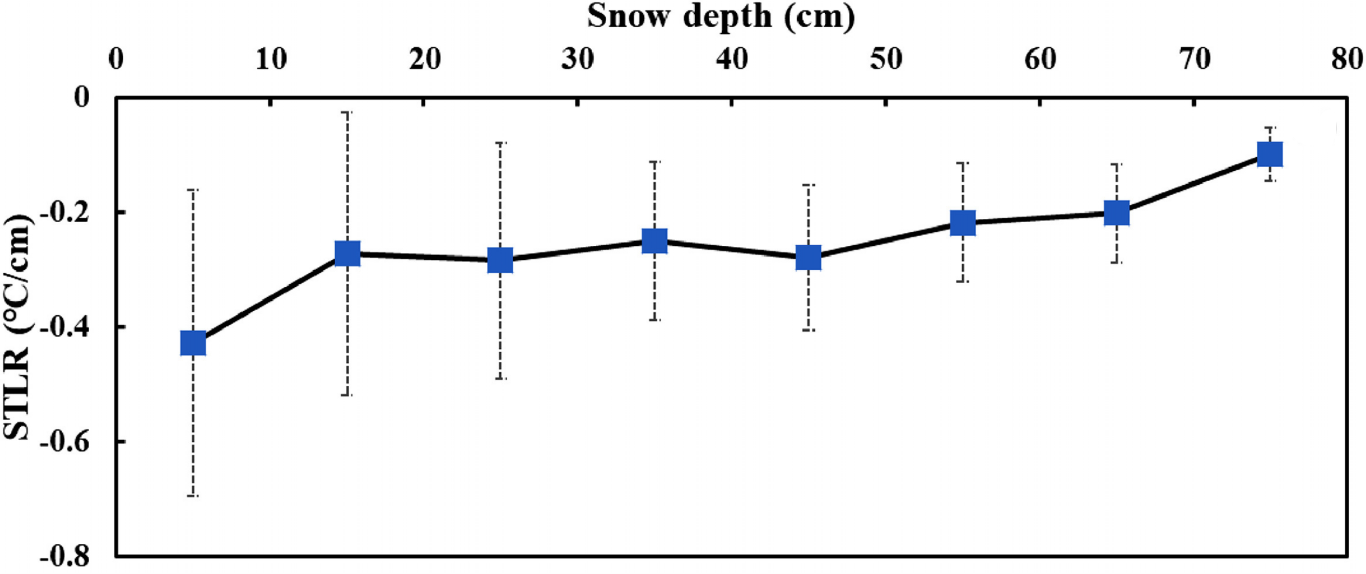
\includegraphics[width=0.95\textwidth]{img/ch1/snowlapserate.png}
	\caption{Teplotní gradient uvnitř sněhové pokrývky v závislosti na její tloušťce. Měřeno na Altaji od listopadu 2011 do dubna 2018. Převzato z \cite{zhangwei2021}.}
	\label{fig:snowlapserate}
\end{figure}

Podle \cite{zhangwei2021} také přítomnost sněhu snižuje teplotu na rozhraní sníh-atmosféra.

Vlhkost vzduchu je pro teplotní gradient v atmosféře důležitou hodnotou. Z hydrostatické rovnice a Poissonových rovnic můžeme odvodit následující vztah\cite{jakvznikapocasi}
\begin{gather*}
-\frac{\text{d}t}{\text{d}z} = \frac{g}{c_p}\frac{T}{T_v},
\end{gather*}
kde $T$ je teplota v kelvinech, $T_v$ je virtuální teplota, $g$ je gravitační zrychlení a $c_p$ je měrné teplo při stálém tlaku. Pak pro suchý vzduch, kde $T=T_v$, dostáváme teplotní gradient $-\frac{\text{d}t}{\text{d}z} = \frac{g}{c_p} = \SI{0.98}{\degree C/100 m}$. Pro stoupající vlhký vzduch je ovšem situace jiná, při výstupu dochází k expanzi, která se děje na úkor vnitřní energie vzduchu. Při chladnutí ve vlhkém vzduchu kondenzuje voda a uvolňuje se skupenské teplo, a tudíž je teplotní gradient menší než v suché atmosféře. Tento gradient závisí na tlaku a teplotě vzduchu. Při tlaku $\SI{1000}{hPa}$ nabývá hodnot $\SI{0.76}{\degree C/100 m}$, $\SI{0.65}{\degree C/100 m}$ a $\SI{0.53}{\degree C/100 m}$ pro $\SI{-10}{\degree C}$ resp. $\SI{0}{\degree C}$, resp. $\SI{10}{\degree C}$\cite{jakvznikapocasi}.

Srážky vedou k nárůstu vlhkosti, jejíž vliv je diskutován výše. Prudký nárůst latentního tepla může výrazně ovlivnit energetickou bilanci poblíž povrchu, jak bylo nastíněno v části \ref{chap:latentheat}. Dále se srážkami typicky roste oblačnost, a tedy klesá množství slunečního záření dopadajícího na zem. Ovšem situace se komplikuje, když vezmeme v potaz roční chod teplot a srážek. Jestliže například v zimě klesají teploty hluboko pod bod mrazu, tak může být vlhkost moc nízká na výskyt srážek, a když už se srážky objeví, znamená to i přísun teplého vzduchu. Teplá advekce v létě typicky znamená advekci vlhkého vzduchu v mimotropických cyklónách, ovšem zároveň může srážky přinést studená fronta a tedy naopak docházet k ochlazení. Studie zabývající se korelací srážek a teploty v Evropě na téměř 100 stanicích zjistila, že v zimě na většině území je významná pozitivní korelace mezi množstvím srážek a teplotou. Pro oblast České republiky a Šumavy je korelace o něco menší a to $0.2$. Pro letní období je pak naopak záporná, tedy s větším množstvím srážek klesají teploty, konkrétně jde o hodnotu okolo $-0.4$\cite{maddenroland1978}.

Insolace je množství záření dopadajícího na horní část zemské atmosféry. Insolace záleží na denní době, roční době a zeměpisné šířce. Okamžitá insolace je dána následujícím vztahem\cite{insolace}
\begin{gather}\label{eq:insolace}
Q = S_0\left(\frac{d_0}{d}\right)^2\left(\sin\phi\sin\delta + \cos\phi\cos\delta\cos h\right),
\end{gather}
kde $S_0$ solární konstanta, $d_0$ je průměrná vzdálenost Země od Slunce, $d$ je aktuální vzdálenost Země od Slunce, $\phi$ je zeměpisná šířka, $\delta$ je deklinační úhel Slunce, $h$ je hodinový úhel Slunce. Tento vzoreček platí pouze pro den, nikoliv v noci, kdy je $Q=0$. Hodinový úhel Slunce spočteme následovně\cite{hourangle}
\begin{equation}
	\begin{split}
		h &= 15^{\circ}\left(\text{LST}+\text{offset}/60-12\right)\\
		\text{offset} &= \text{eot} + \text{longV}\\
		\text{eot} &= 229.18\cdot(0.000075+0.001868\cos(\gamma)-0.032077\sin(\gamma)\\
		& -0.014615\cos(2\gamma)-0.040849\sin(2\gamma))\\
		\text{longV} &= 4\cdot\text{longitude}\qquad \gamma = \frac{2\pi}{365}\left(t - 1 + \frac{\text{hour}-12}{24}\right),
	\end{split}
\end{equation}
kde $\text{LST}$ je místní sluneční čas, ke kterému přičteme korekci způsobenou eliptickou dráhou okolo země a skloněním zemského osy a korekci zahrnující to na jaké zeměpisné šířce se nacházíme. Faktor $\gamma$ je část roku vyjádřena ve zlomku.
Deklinační úhel s předpokladem, že Země obíhá po kružnici\cite{declinationangle}
\begin{gather*}
\delta = \SI{-23.45}{\degree} \cdot \cos\left(\frac{360}{365}\cdot(t+10)\right),
\end{gather*}
kde $t$ je den v roce, tedy pro 1. leden $t=1$. Vzdálenost Země od Slunce pro \eqref{eq:insolace} je daná vztahem\cite{sunearthdist}
\begin{gather*}
d = 1-0.01672\cdot \cos\left(0.9856\cdot(t-4)\right)
\end{gather*}

V praktické části práce budeme analyzovat, jaký vliv mají tyto proměnné na rozdíl mezi teplotou naměřenou v lesním porostu v Národním parku Šumava a Národním parku Bavorský les ve výšce $\SI{2}{m}$ a při povrchu, tedy $\SI{0}{cm}$ a $\SI{15}{cm}$.

\section{Popis měření meteorologický veličin} \label{chap:measure}
\subsection{Měření na meteorologických stanicích}
Teplota vzduchu by podle Světové meteorologické organizace (WMO) měla být měřena ve výšce $\SI{1.25}{m}$ až $\SI{2}{m}$\cite{wmoGuidance2021}. V České republice Český hydrometeorologický ústav provozuje celou řadu meteorologických stanic různého charakteru s různými měřenými meteorologickými proměnnými. Měření na stanicích probíhá následujícím způsobem. Stanice by měla být na trávníku nikoliv například na asfaltu a měření probíhají v pravidelných intervalech. Pro synoptické stanice je to například v takzvaných hlavních termínech ($00$, $06$, $12$ a $18$ UTC) a případně vedlejších ($03$, $09$, $15$, $21$ hodin UTC). Na stanicích jsou měřeny veličiny jako například, vlhkost, výška sněhu, část zatažené oblohy, tlak a další\cite{chmustanice}. 

\subsection{Měření v terénu pomocí čidel}
Pomocí meteorologických stanic není možné získat detailní informace o teplotě a dalších veličinách na malých prostorových škálách. Standardní meteorologické stanice nemůžou změřit teplotu například v lesním porostu. Data použitá v této práci jsou měřená pomocí TMS (Temperature-Moisture-Sensor) logger. Kromě čidel jako například Thermochron iButtons, je možné využít radiometrie a z vyzářeného záření z povrchu pomocí Stefan-Boltzmannova zákona spočítat teplotu povrchu. Poslední metoda má ovšem své omezení pokud chceme znát teplotu v lesním porostu. 

\subsubsection{TMS4 a T1 logger} \label{chap:loggers}
Čidlo TMS4 logger používané pro sběr dat vědci a vědkyněmi z Botanického ústavu Akademie věd České republiky je konstruováno tak, aby měřilo podmínky, které prožívá malá bylina. Je tedy vysoké $\SI{15}{cm}$ a sahá do hloubky $\SI{14}{cm}$. Je opatřeno třemi teplotními senzory ve výškách $\SI{15}{cm},\ \SI{0}{cm},\ \SI{-8}{cm}$. Až do hloubky $\SI{14}{cm}$ je měřena volumetrická půdní vlhkost. Všechny hodnoty jsou měřeny v 15-ti minutových intervalech. Vršek data loggeru je opatřen optickým stíněním z bílého plastu chránící horní senzor před přímým slunečním zářením a stejně tak je odstíněn i senzor při povrchu země. 

Teplotní senzor měří s přesností $\SI{\pm 0.5}{\degree C}$ a funguje na intervalu $\SI{-55}{\degree C}$ až $\SI{125}{\degree C}$. Měření volumetrické půdní vlhkostí je založené na time-domain-transmission (TDT), kdy jsou skrze obvod vysílány elektromagnetické pulzy a množství detekovaných pulzů je přímo úměrné vlhkosti. 

Při srovnání TMS4 loggeru se standardní meteorologickou stanicí typu METEOS 5 byla pozorována větší variabilita u teplot v $\SI{15}{cm}$ než ve $\SI{2}{m}$. TMS4 loggeru byl instalován na krátkém posekaném trávníku, tři metry od stanice, a rozdíl teplot při hodinovém měření se pohyboval od $\SI{+8.45}{\degree C}$ do $\SI{-6.05}{\degree C}$. Průměrné denní teploty naměřené z TMS4 loggeru byly systematicky nižší, průměrný rozdíl ovšem pouze $\SI{-0.58}{\degree C}$, v zimě jsou tyto rozdíly větší a to $\SI{-2.02}{\degree C}$ až $\SI{0.6}{\degree C}$. Opačný trend pak můžeme pozorovat, pokud není teplotní senzor v $\SI{15}{cm}$ odstíněn plastovým krytem. V létě byly teploty nižší až o $\SI{5.08}{\degree C}$, ale v zimě byly podobné. Teploty z půdních senzorů jak TMS4 loggeru tak stanice METEOS 5 se lišily velmi málo, rozdíl mezi naměřenými teplotami byl tedy zřejmě způsoben primárně polohou senzorů a použitým stíněním než jejich typem. Rozdíly mezi naměřenými teplotami nad zemí byly ještě výraznější pro proměnné, které jsou často používány v ekologických studiích, jako například kvantily extrémních teplot\cite{WildJan2019Caer}. 

Data měřená při povrchu země jsou na některých místech doplněna stejnými teplotními senzory ve výšce $\SI{2}{m}$ upevněnými na kmenu stromu a také opatřena plastovým stínítkem.

\section{Národní park Šumava a Bavorský les} \label{chap:sumavabavorskyles}
Čidla TMS logger z kterých pocházejí data použitá v této práci se nacházejí v oblasti Národního parku Šumava o rozloze $\SI{68 064}{ha}$\cite{npsumava} a Národního parku Bavorský les, $\SI{24 250}{ha}$.

\subsection{Geologie}
Šumava patří mezi nejstarší pohoří ve střední Evropě\cite{WildJan2004Cops}. Typické horniny Šumavy jsou přeměněné horniny a to především ruly a vyvřelé horniny, zejména granity. Dále zde nalezneme uloženiny jako jsou rašeliny, ale i sedimenty ledovcového původu. Svahové sedimenty jsou pak tvořeny hlínami, hlinitými písky, hlinito-kamenitými sedimenty a blokovými sedimenty. Nejvyšším bodem NP Šumava je Plechý $\SI{1378}{m.\ n.\ m.}$, Šumavské pláně ve výšce $\SI{1000}{m.\ n.\ m.}$ tvoří hlavní část národního parku\cite{npsumava}. Většina pohoří na české straně náleží povodí Labe a tedy řekám Vltava a Otava.

Nejvyšší bod Národního parku Bavorský les je Großer Rachel (česky Roklan) o výšce $\SI{1453}{m.\ n.\ m.}$, povodí většiny Bavorského lesa je Černé moře.

\subsection{Klima}
Průměrná teplota se pohybuje od $\SI{6}{\degree C}$ ve výšce $\SI{750}{m.\ n.\ m.}$ do $\SI{3}{\degree C}$ ve výšce $\SI{1300}{m.\ n.\ m.}$. Rekordně nejnižší teplota v NP Šumava byla naměřena v Jezerní slati a to $\SI{-41.6}{\degree C}$. Roční úhrn srážek se pohybuje ve velkém rozmezí od $\SI{800}{mm}$ až po ojedinělých $\SI{1600}{mm}$. Prostorové rozložení pak můžeme vidět na obrázku \ref{fig:srazkovepomerysumava} s významné rostoucími srážky pro vyšší oblasti Šumavy, obdobně můžeme vidět rozložení srážek pro Bavorsko a Bavorský les na obrázku \ref{fig:srazkovepomerybavorskyles}. Sněhová pokrývka se pohybuje mezi $\SI{40}{cm}$ až $\SI{150}{cm}$ a drží se 120 až 150 dní\cite{npsumava}.

\begin{figure}
	\centering
	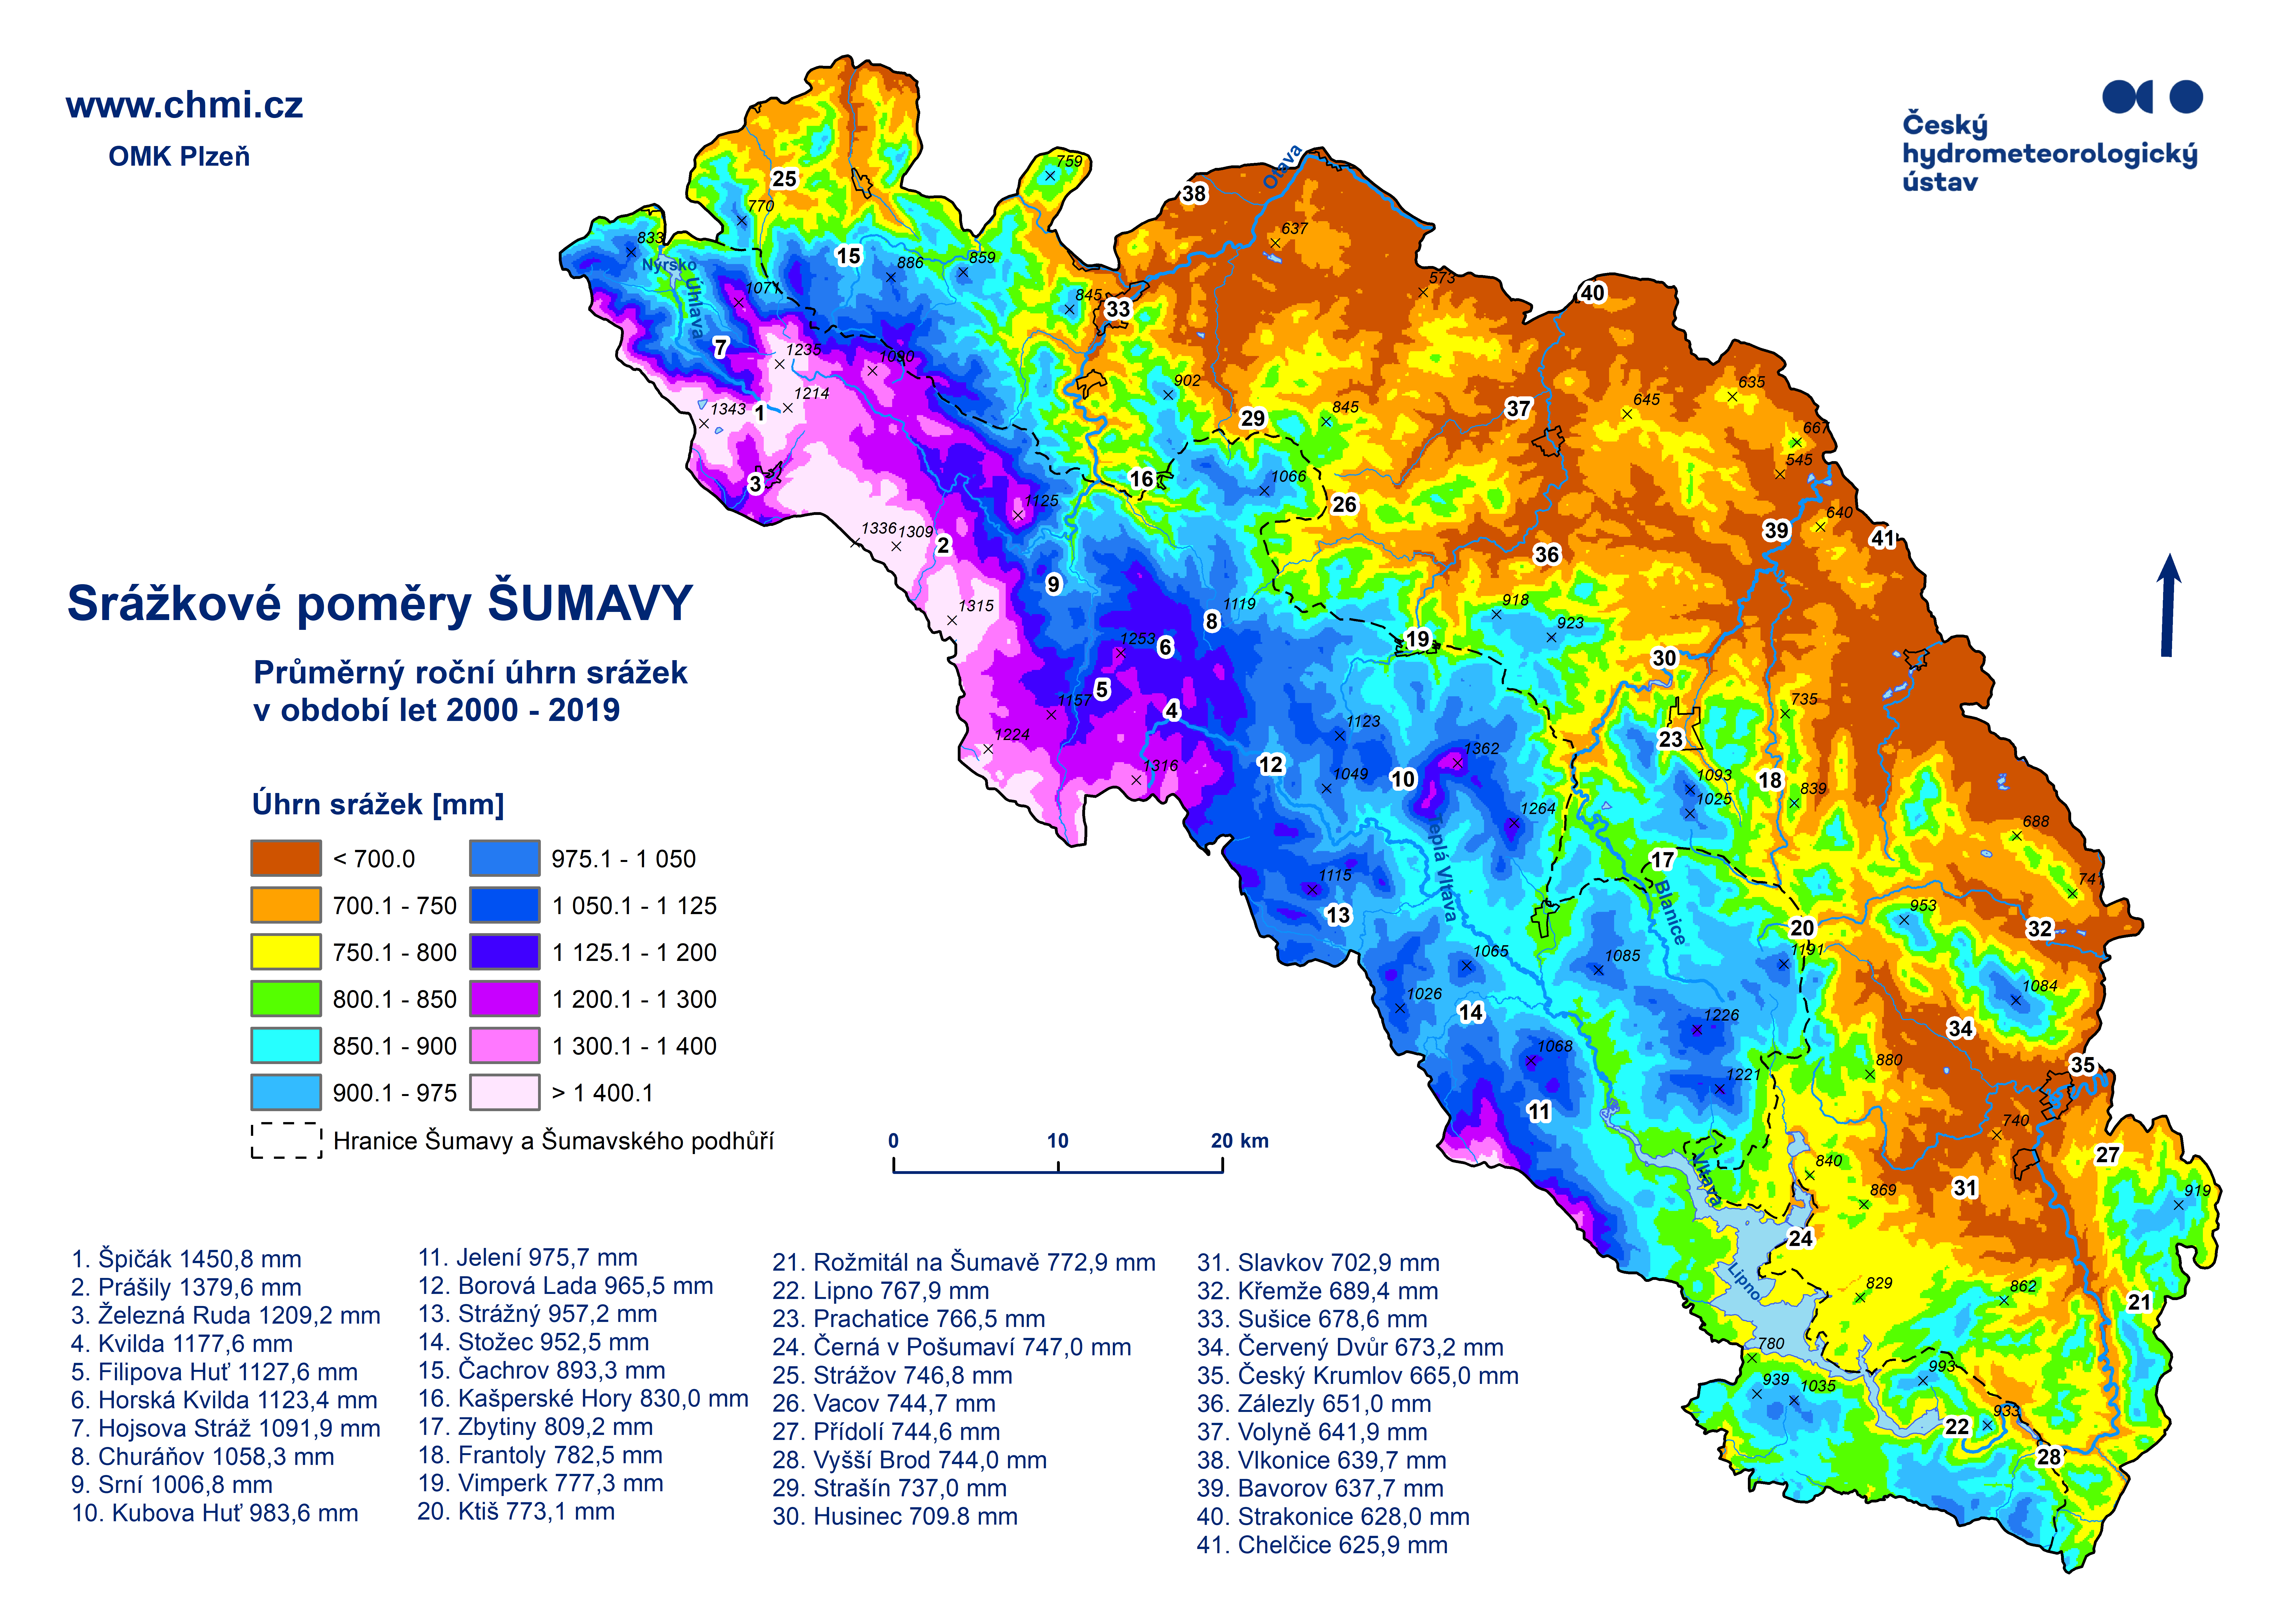
\includegraphics[width=0.95\textwidth]{img/ch1/srazkovepomerysumava.png}
	\caption{Srážkové poměry Šumavy\cite{srazkovepomerysumava}, důležitá je pak hodnota $\SI{1058}{mm/rok}$ pro meteorologickou stanici Churáňov.}
	\label{fig:srazkovepomerysumava}
\end{figure}

\begin{figure}
	\centering
	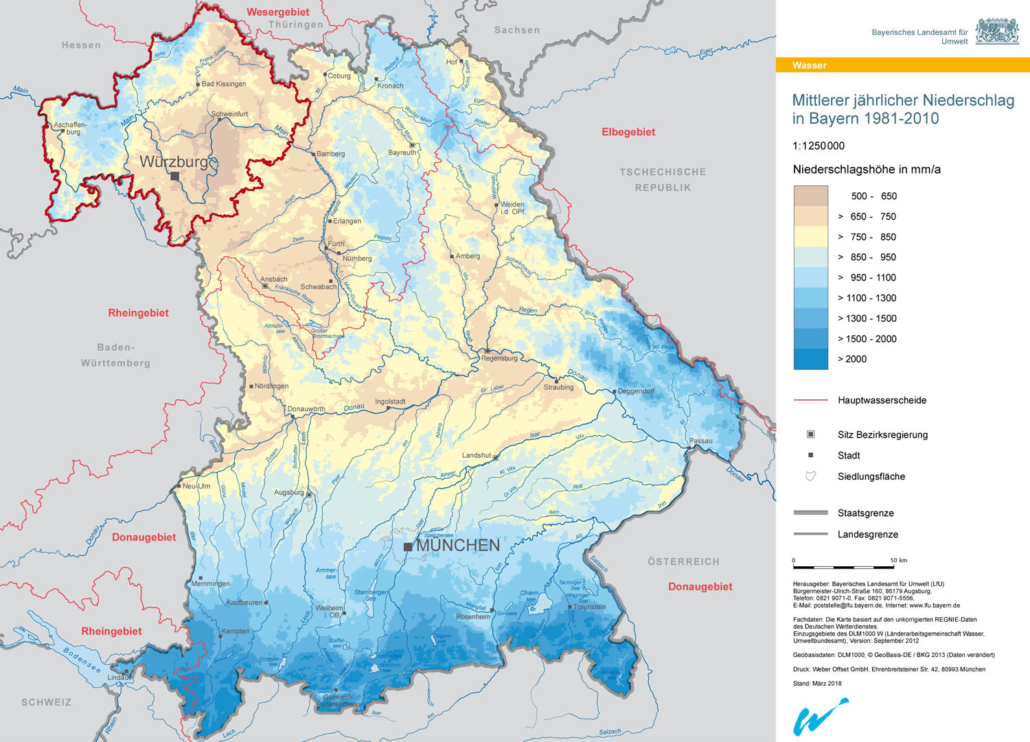
\includegraphics[width=0.95\textwidth]{img/ch1/srazkovepomerybavorskyles.png}
	\caption{Srážkové poměry v Bavorsku\cite{srazkovepomerybavorskyles}}
	\label{fig:srazkovepomerybavorskyles}
\end{figure}

Více než $\SI{80}{\%}$ území NP Šumava pokrývá les. Typické pro toto území jsou horské smrčiny, smrkové a bukové pralesy. Nacházejí se zde i rašeliniště a louky.

\section{Statistické metody}\label{chap:statistika}
V kapitole \ref{chap:analysis} je vysvětleno jakým způsobem byla data zpracována. Zde nastíníme relevantní teorii.

\subsection{Lineární smíšený model}
V maticovém zápisu je lineární smíšený model definován následovně\cite{mcleanrobert1991}
$$\boldsymbol{y} = \boldsymbol{X}\boldsymbol{\beta} + \boldsymbol{Z}\boldsymbol{u} + \boldsymbol{\epsilon},$$ \label{eq:linearmixedeffectmodel}
kde $\mathbf{y}$ je vektor pozorovaných hodnot, $\mathbf{\beta}$ je neznámý vektor hledaných fixní efektů, $\mathbf{u}$ je neznámý vektor náhodných efektů $\mathbf{\epsilon}$ je neznámý vektor náhodných chyb a matice $\mathbf{X}$ a $\mathbf{Z}$ jsou známé matice udávající vztah mezi pozorovanými hodnotami a fixními, resp. náhodnými efekty, jejichž velikost je daná počtem prediktorů a pozorování\cite{mcleanrobert1991}.

Předpokládáme u lineárního smíšeného modelu normální rozdělení residuí a očekáváme homoskedasticitu, tedy to, že rezidua nezávisí na hodnotě měřené veličiny. Dále také předpokládáme data bez autokorelační struktury. Jak ovšem uvidíme v kapitole \ref{chap:analysis}, tak naše data vykazují časovou korelační strukturu. Další předpoklad je normální rozdělení náhodný efektů modelu\cite{hefleytrevorj2017}. 

Pro modelování autokorelační struktury můžeme využít ARMA (autoregressive-moving-average) model. Ten je definován jako\cite{wilsongranville2016}
$$y_T = \epsilon_T + \sum_{i=1}^{p}u_i y_{T-i} + \sum_{i=1}^{q}\beta_i\varepsilon_{T-i}$$,
kde $y_T$ časová řada, $\epsilon$ je náhodná chyba, $u_i$ jsou parametry náhodné proměnné a $\beta_i$ jsou parametry fixní proměnné. 
